% Ch.7 Main Results (~12-15 pp). Draft Days 5-7 (one phase per day).
\chapter{Main Results}
\label{ch:results}

% --- Phase I ----------------------------------------------------------------
\section{Phase I: The Local Cycle Factor across G10}
\label{sec:res-phase1}
% Eq (18): rx_{i,t+12} = alpha_i + beta_i CF_{i,t} + eps. Per-country
% predictability; signs/magnitudes; R^2 across countries and maturities.
\begin{figure}[t]\centering
  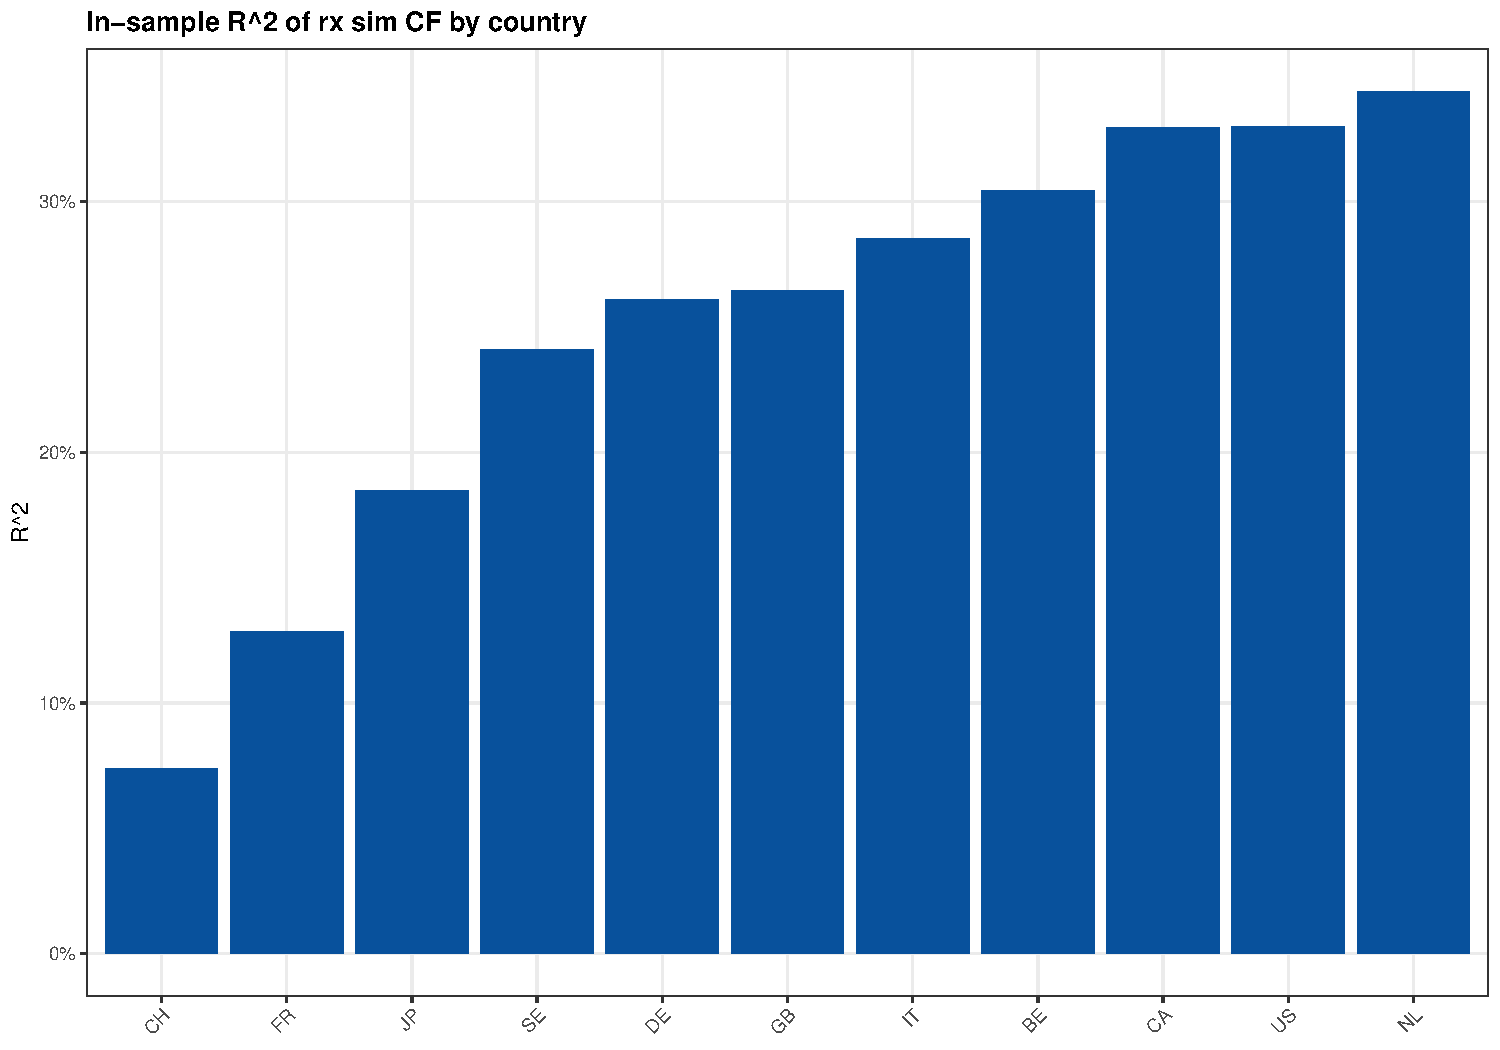
\includegraphics[width=0.9\linewidth]{figures/s4_r2_cf_by_country.pdf}
  \caption{In-sample $R^2$ of the local cycle factor, by country.}
  \label{fig:s4-r2}
\end{figure}

% --- Phase II ---------------------------------------------------------------
\section{Phase II: Does the Global Factor Subsume the Local Factor?}
\label{sec:res-phase2}
% Eq (19)-(20) horse race: rx ~ CF + GCF vs rx ~ GCF. Orthogonalized local CF,
% joint Wald tests, BH-FDR (plots.R s5_*, s9_*).
\begin{figure}[t]\centering
  
\includegraphics[width=0.9\linewidth]{figures/s5_r2_cf_vs_gcf.pdf}
  \caption{Local vs global cycle factor: predictive $R^2$.}
  \label{fig:s5-r2}
\end{figure}
\begin{figure}[t]\centering
  
\includegraphics[width=0.9\linewidth]{figures/s9_hr_wald.pdf}
  \caption{Horse-race Wald tests: local vs global factor.}
  \label{fig:s9-wald}
\end{figure}

% --- Phase III --------------------------------------------------------------
\section{Phase III: The Global Investor and the FX-Adjusted Factor}
\label{sec:res-phase3}
% Eq (21)-(23): USD-investor returns; does currency risk break the model; does
% the FX-adjusted FXGCF restore predictability? (plots.R s6_*; DH Table 7.)
\begin{figure}[t]\centering
  
\includegraphics[width=0.9\linewidth]{figures/s6_r2_usd_gcf_vs_fxgcf.pdf}
  \caption{USD-investor returns: GCF vs FX-adjusted FXGCF.}
  \label{fig:s6-r2}
\end{figure}

\section{Summary of Findings}
\label{sec:res-summary}
% Tie back to the research questions; bridge to robustness.
